The analysis uses a uniform tube of length $L$ with a closed end at $x=0$ and an open end at $x=L$. The acoustic displacement is $u(x,t)$ and the pressure disturbance is $p(x,t)$. The derivation follows the course notes (pp. 114--118) for harmonic vibration with $\omega>0$.

\textbf{1. Tube sketch.} The closed wall imposes zero particle displacement, while the open end imposes zero pressure disturbance. The tube contains a fluid with area $A$, density $\rho$, bulk modulus $K$, and wave speed $c$.

\begin{figure}[H]
\centering
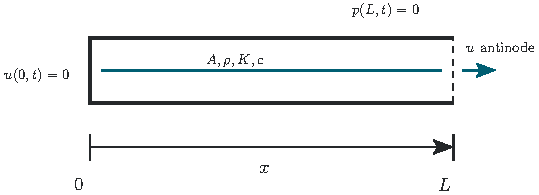
\includegraphics[width=0.84\linewidth]{figures/generated/solutions/C1-tube.pdf}
\caption{Closed--open tube used for the analysis. The closed end is at $x=0$ and the open end is at $x=L$.}
\label{fig:hw02-c1-tube}
\end{figure}

\textbf{2. Boundary conditions.} At the closed end the fluid cannot move, and at the open end the pressure disturbance vanishes.
\[
\boxed{u(0,t)=0},\qquad \boxed{p(L,t)=0}.
\]

\textbf{3. Harmonic displacement solution.} Separation of variables gives
\[
\boxed{u(x,t)=U(x)e^{-i\omega t}},\qquad
\boxed{U(x)=C_1\sin(\gamma x)+C_2\cos(\gamma x)}.
\]

\textbf{4. Pressure--displacement relation.} The pressure disturbance is related to the axial strain by
\[
\boxed{p(x,t)=-K\frac{\partial u}{\partial x}}.
\]

\textbf{5. Pressure in terms of $C_1$ and $C_2$.} Differentiating the displacement field gives
\[
\boxed{p(x,t)=-K\gamma\left[C_1\cos(\gamma x)-C_2\sin(\gamma x)\right]e^{-i\omega t}}.
\]

\begin{samepage}
\textbf{6. Boundary equations.} Substitution into the boundary conditions gives
\[
u(0,t)=C_2e^{-i\omega t}=0,
\]
\[
p(L,t)=-K\gamma\left[C_1\cos(\gamma L)-C_2\sin(\gamma L)\right]e^{-i\omega t}=0.
\]
\end{samepage}

\textbf{7. Constants.} The first equation gives $C_2=0$. The second equation then becomes
\[
\boxed{C_1\cos(\gamma L)=0}.
\]

\textbf{8. Trivial solution.} If $C_1=0$, then $C_2=0$ also, so $U(x)=0$, $u(x,t)=0$, and $p(x,t)=0$. This is the fluid at rest and contains no vibration.

\textbf{9. Nontrivial solution.} For vibration, take $C_1\ne0$. The wavenumber must therefore satisfy
\[
\boxed{\cos(\gamma L)=0}.
\]

\textbf{10. Eigenvalue equation.} With $z=\gamma L$,
\[
\boxed{\cos z=0}.
\]

\textbf{11. Eigenvalues.} The positive roots are
\[
\boxed{z_j=\frac{(2j-1)\pi}{2}},\qquad j=1,2,3,\ldots.
\]

\textbf{12. Wavenumbers.} Since $z_j=\gamma_jL$,
\[
\boxed{\gamma_j=\frac{(2j-1)\pi}{2L}}.
\]

\textbf{13. Wavenumber definition.} The wavenumber is related to angular frequency by
\[
\boxed{\gamma=\frac{\omega}{c}}.
\]

\textbf{14. Angular frequency.} Solving the preceding relation for frequency gives
\[
\boxed{\omega=\gamma c}.
\]

\textbf{15. Natural angular frequencies.} Substituting $\gamma_j$ gives
\[
\boxed{\omega_j=\frac{(2j-1)\pi c}{2L}}.
\]

\textbf{16. Frequencies in hertz.} Since $\omega_j=2\pi f_j$,
\[
\boxed{f_j=\frac{(2j-1)c}{4L}}.
\]

\textbf{17. Fundamental and overtones.} The fundamental frequency is $f_1=c/(4L)$. The overtones are the higher resonant frequencies. Here $f_2=3f_1$ is the first overtone, $f_3=5f_1$ is the second overtone, and in general $f_j=(2j-1)f_1$.

\textbf{18. Harmonics.} The fundamental is the first harmonic. The closed--open tube supports only odd harmonics, so the first overtone is the third harmonic, the second overtone is the fifth harmonic, and no even harmonics occur in this ideal model.

\textbf{19. Wavelength relation.} Wavenumber and wavelength satisfy
\[
\boxed{\lambda=\frac{2\pi}{\gamma}}.
\]

\textbf{20. Modal wavelengths.} Using the wavenumbers above,
\[
\boxed{\lambda_j=\frac{4L}{2j-1}}.
\]

\textbf{21. Wavelength multiples.} Rearranging the last expression gives
\[
\boxed{L=(2j-1)\frac{\lambda_j}{4}}.
\]
Thus the tube contains one, three, five, and so on quarter-wavelengths. The closed end is a displacement node and a pressure antinode, while the open end is a displacement antinode and a pressure node.

\textbf{22. Elimination of $C_2$.} From item 7, $C_2=0$, so
\[
\boxed{U(x)=C_1\sin(\gamma x)}.
\]

\textbf{23. Displacement modeshapes.} Choosing the arbitrary scale $C_1=1$ gives
\[
\boxed{U_j(x)=\sin(\gamma_jx)=\sin\left(\frac{(2j-1)\pi x}{2L}\right)}.
\]

\textbf{24. Normalized displacement modeshapes.} The first five modes are plotted against $\xi=x/L$ in Figure~\ref{fig:hw02-c1-disp}. All modes have a node at $\xi=0$ and an antinode at $\xi=1$. The five modes fit one, three, five, seven, and nine quarter-wavelengths into the tube. Mode $j$ has $j$ displacement nodes, including the closed end, and $j$ antinodes, including the open end.

\begin{figure}[H]
\centering
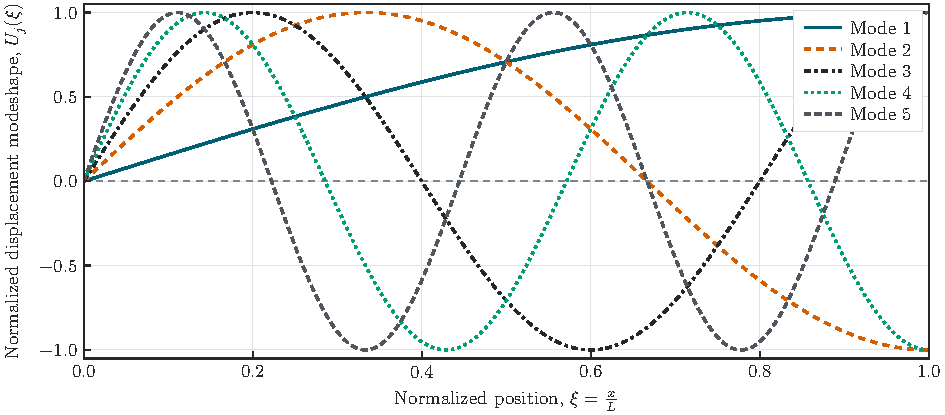
\includegraphics[width=0.96\linewidth]{figures/generated/solutions/C1-modes.pdf}
\caption{Normalized displacement modeshapes $U_j(\xi)=\sin((2j-1)\pi\xi/2)$ for the first five closed--open tube modes.}
\label{fig:hw02-c1-disp}
\end{figure}

\textbf{25. Graduate work.} Let $a_j>0$ denote the displacement amplitude in meters. Using $u_j(x,t)=a_jU_j(x)e^{-i\omega_jt}$ with $p=-Ku_x$ gives
\[
p_j(x,t)=-K a_j\gamma_j\cos(\gamma_jx)e^{-i\omega_jt}.
\]
Normalizing by the peak pressure amplitude $K a_j\gamma_j$ gives
\[
\boxed{\bar P_j(\xi)=-\cos\left(\frac{(2j-1)\pi\xi}{2}\right)}.
\]
The pressure modeshapes are plotted in Figure~\ref{fig:hw02-c1-pressure}. The closed end is a pressure antinode and a displacement node. The open end is a pressure node and a displacement antinode. Mode $j$ has $j$ pressure nodes and $j$ pressure antinodes, with the endpoint roles reversed from displacement. The displacement and pressure fields remain related by differentiation, so the negative sign preserves $p=-Ku_x$.

\begin{figure}[H]
\centering
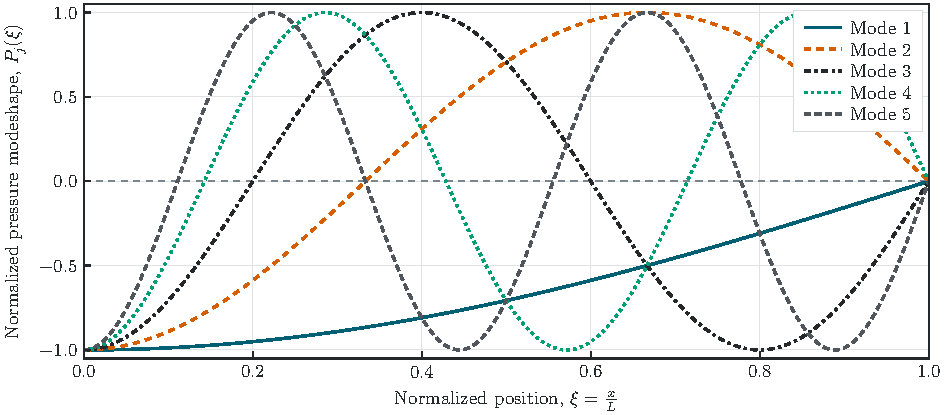
\includegraphics[width=0.96\linewidth]{figures/generated/solutions/C1-pressure.pdf}
\caption{Normalized pressure modeshapes $\bar P_j(\xi)=-\cos((2j-1)\pi\xi/2)$ for the first five closed--open tube modes.}
\label{fig:hw02-c1-pressure}
\end{figure}

\clearpage
\matlabcaption{MATLAB plots for C.1.}
\lstinputlisting[style=hwmatlab]{matlab/C1.m}
